\documentclass[
	12pt,
	a4paper,
	bibtotoc,
	cleardoubleempty, 
	idxtotoc,
	ngerman,
	openright
	final,
	listof=nochaptergap,
	]{scrbook}

\usepackage[T1]{fontenc}
\usepackage[ansinew]{inputenc}

% ##################################################
% Unterstuetzung fuer die deutsche Sprache
% ##################################################
\usepackage{ngerman}
\usepackage[ngerman]{babel}
\usepackage{graphicx}
\usepackage{float}

% ##################################################
% Dokumentvariablen
% ##################################################

% Persoenliche Daten
\newcommand{\docNachname}{BERNER}
\newcommand{\docVorname}{FABIAN}
\newcommand{\docStrasse}{ROBERT-GERWIG-PLATZ 1}
\newcommand{\docOrt}{FURTWANGEN}
\newcommand{\docPlz}{78120}
\newcommand{\docEmail}{FABIAN.BERNER@hs-furtwangen.de}
\newcommand{\docMatrikelnummer}{1 4 8 15 16 23 42}

% Dokumentdaten
\newcommand{\docTitle}{TITEL}
%\newcommand{\docUntertitle}{} % Kein Untertitel
\newcommand{\docUntertitle}{UNTERTITEL}
% Arten der Arbeit: Bachelorthesis, Masterthesis, Seminararbeit, Diplomarbeit
\newcommand{\docArtDerArbeit}{ART DER ARBEIT}
%Studiengaenge: Allgemeine Informatik Bachelor, Computer Networking Bachelor,
% Software-Produktmanagement Bachelor, Advanced Computer Scinece Master
\newcommand{\docStudiengang}{STUDIENGANG}
\newcommand{\docAbgabedatum}{11.11.2011}
\newcommand{\docErsterReferent}{ERSTER REFERENT}
%\newcommand{\docZweiterReferent}{-} % Wenn es nur einen Betreuer gibt
\newcommand{\docZweiterReferent}{ZWEITER REFERENT}

% ##################################################
% Allgemeine Pakete
% ##################################################

% Abbildungen einbinden
\usepackage{graphicx}
\usepackage{float}

% Zusaetsliche Sonderzeichen
\usepackage{dingbat}

% Farben
\usepackage{color}
\usepackage[usenames,dvipsnames,svgnames,table]{xcolor}

% Maskierung von URLs und Dateipfaden
\usepackage[hyphens]{url}

% Deutsche Anfuehrungszeichen
\usepackage[babel, german=quotes]{csquotes}

% Pakte zur Index-Erstellung (Schlagwortverzeichnis)
\usepackage{index}
\makeindex

% Ipsum Lorem
% Paket wird nur für das Beispiel gebraucht und kann gelöscht werden
\usepackage{lipsum}

% ##################################################
% Seitenformatierung
% ##################################################
\usepackage[
	portrait,
	bindingoffset=1.5cm,
	inner=2.5cm,
	outer=2.5cm,
	top=3cm,
	bottom=2cm,
	%includeheadfoot
	]{geometry}

% ##################################################
% Kopf- und Fusszeile
% ##################################################

\usepackage{fancyhdr}

\pagestyle{fancy}
\fancyhf{}
\fancyhead[EL,OR]{\sffamily\thepage}
\fancyhead[ER,OL]{\sffamily\leftmark}

\fancypagestyle{headings}{}

\fancypagestyle{plain}{}

\fancypagestyle{empty}{
  \fancyhf{}
  \renewcommand{\headrulewidth}{0pt}
}

%Kein "Kapitel # NAME" in der Kopfzeile
\renewcommand{\chaptermark}[1]{
	\markboth{#1}{}
   	\markboth{\thechapter.\ #1}{}
}

%Einr�cken von Abs�tzen deaktivieren
\setlength{\parindent}{0pt}

%Zeilenabstand bei abst�tzen
\usepackage{parskip}

% ##################################################
% Schriften
% ##################################################

% Stdandardschrift festlegen
\renewcommand{\familydefault}{\sfdefault}

% Standard Zeilenabstand: 1,5 zeilig
\usepackage{setspace}
\onehalfspacing 

% Schriftgroessen festlegen
\addtokomafont{chapter}{\sffamily\large\bfseries} 
\addtokomafont{section}{\sffamily\normalsize\bfseries} 
\addtokomafont{subsection}{\sffamily\normalsize\mdseries} 
\addtokomafont{caption}{\sffamily\normalsize\mdseries} 

% ##################################################
% Inhaltsverzeichnis / Allgemeine Verzeichniseinstellungen
% ##################################################

\usepackage{tocloft}

% Punkte auch bei Kapiteln
\renewcommand{\cftchapdotsep}{3}
\renewcommand{\cftdotsep}{3}

% Schriftart und -groesse im Inhaltsverzeichnis anpassen
\renewcommand{\cftchapfont}{\sffamily\normalsize}
\renewcommand{\cftsecfont}{\sffamily\normalsize}
\renewcommand{\cftsubsecfont}{\sffamily\normalsize}
\renewcommand{\cftchappagefont}{\sffamily\normalsize}
\renewcommand{\cftsecpagefont}{\sffamily\normalsize}
\renewcommand{\cftsubsecpagefont}{\sffamily\normalsize}

%Zeilenabstand in den Verzeichnissen einstellen
\setlength{\cftparskip}{.5\baselineskip}
\setlength{\cftbeforechapskip}{.1\baselineskip}

% ##################################################
% Abbildungsverzeichnis und Abbildungen
% ##################################################

\usepackage{caption}
\usepackage{float}
\usepackage{wrapfig}

% Nummerierung von Abbildungen
\renewcommand{\thefigure}{\arabic{figure}}
\usepackage{chngcntr}
\counterwithout{figure}{chapter}

% Abbildungsverzeichnis anpassen
\renewcommand{\cftfigpresnum}{Abbildung }
\renewcommand{\cftfigaftersnum}{:}

% Breite des Nummerierungsbereiches [Abbildung 1:]
\newlength{\figureLength}
\settowidth{\figureLength}{\bfseries\cftfigpresnum\cftfigaftersnum}
\setlength{\cftfignumwidth}{\figureLength}
\setlength{\cftfigindent}{0cm}

% Schriftart anpassen
\renewcommand\cftfigfont{\sffamily}
\renewcommand\cftfigpagefont{\sffamily}

% ##################################################
% Tabellenverzeichnis und Tabellen
% ##################################################

% Nummerierung von Tabellen
\renewcommand{\thetable}{\arabic{table}}
\counterwithout{table}{chapter}

% Tabellenverzeichnis anpassen
\renewcommand{\cfttabpresnum}{Tabelle }
\renewcommand{\cfttabaftersnum}{:}

% Breite des Nummerierungsbereiches [Abbildung 1:]
\newlength{\tableLength}
\settowidth{\tableLength}{\bfseries\cfttabpresnum\cfttabaftersnum}
\setlength{\cfttabnumwidth}{\tableLength}
\setlength{\cfttabindent}{0cm}

%Schriftart anpassen
\renewcommand\cfttabfont{\sffamily}
\renewcommand\cfttabpagefont{\sffamily}

% Unterdrueckung von vertikalen Linien
\usepackage{booktabs}

% ##################################################
% Listings (Quellcode)
% ##################################################

\usepackage{listings}
\lstset{
	language=java,
	backgroundcolor=\color{white},
	breaklines=true,
	prebreak={\carriagereturn},
 	breakautoindent=true,
 	numbers=left,
 	numberstyle=\tiny,
 	stepnumber=2,
 	numbersep=5pt,
 	keywordstyle=\color{blue},
   	commentstyle=\color{green},   
   	stringstyle=\color{gray}
}
  	
% ##################################################
% Theoreme
% ##################################################
  	
% Umgebung fuer Beispiele
\newtheorem{beispiel}{Beispiel}

% Umgebung fuer These
\newtheorem{these}{These}

% Umgebung fuer Definitionen
\newtheorem{definition}{Definition}
  	
% ##################################################
% Literaturverzeichnis
% ##################################################

\usepackage{bibgerm}

% ##################################################
% Abkuerzungsverzeichnis
% ##################################################

\usepackage[printonlyused]{acronym}

% ##################################################
% PDF / Dokumenteninternelinks
% ##################################################

\usepackage[
	colorlinks=false,
   	linkcolor=black,
   	citecolor=black,
  	filecolor=black,
	urlcolor=black,
    bookmarks=true,
    bookmarksopen=true,
    bookmarksopenlevel=3,
    bookmarksnumbered,
    plainpages=false,
    pdfpagelabels=true,
    hyperfootnotes,
    pdftitle ={\docTitle},
    pdfauthor={\docVorname~\docNachname},
    pdfcreator={\docVorname~\docNachname}]{hyperref}

\begin{document}

\setcounter{secnumdepth}{3}

% Titelblatt
\begin{titlepage}
\pagestyle{empty}

% ##################################################
% HFU-Logo einbinden
% ##################################################
\begin{flushright}
\begin{figure}[ht]
\flushright

\includegraphics[height=3cm]{content/pictures/hfu.jpg}
\end{figure}
\end{flushright}

% ##################################################
% Titel
% ##################################################
\begin{center}
{\fontsize{18}{22} \selectfont Dokumentation des Projekts}\\[5mm]
{\fontsize{18}{22} \selectfont im Studiengang} \\[5mm]
{\fontsize{18}{22} \selectfont AIB}\\
\vspace{1cm}
\begin{onehalfspace}
{\fontsize{22}{26} \selectfont \textbf{DiceWars}}\\[5mm]



\end{onehalfspace}
\end{center}

% ##################################################
% Zusatzinformationen
% ##################################################
\vfill
\begin{center}
\begin{tabular}{lcl}
Referent  		&:& Prof. Dr. Gerd Unruh 	\\ \\
%Koreferent 		&:& \docZweiterReferent \\ \\	
Vorgelegt am 	&:& 09.06.2015	\\ \\
Vorgelegt von 	&:& E.Albach, M.Haas, J.Preu�, P.Polster \\
				& & eduard.albach@hs-furtwangen.de \\
				& &	marco.haas@hs-furtwangen.de	\\
				& & jan-henrik.preuss@hs-furtwangen.de\\
				& & phillip.polster@hs-furtwangen.de	
\end{tabular}
\end{center}
\end{titlepage}
\cleardoubleemptypage

\frontmatter


% Abstract

\cleardoubleemptypage

% Inhaltsverzeichnis
\tableofcontents
\addcontentsline{toc}{chapter}{Inhaltsverzeichnis}
\cleardoubleemptypage

% Abbildungsverzeichnis einbinden und ins Inhaltsverzeichnis
% WORKAROUND: tocloft und KOMA funktionieren zusammen nicht
% korrekt\phantomsection
%\addcontentsline{toc}{chapter}{\listfigurename} 
%\listoffigures
\cleardoubleemptypage

% Tabellenverzeichnis einbinden und ins Inhaltsverzeichnis
% WORKAROUND: tocloft und KOMA funktionieren zusammen nicht
% korrekt\phantomsection
\phantomsection
%\addcontentsline{toc}{chapter}{\listtablename}
%\listoftables
\cleardoubleemptypage

% Abkürzungsverzeichnis


\mainmatter


\chapter{Einleitung}  
F�r die Durchf�hrung des Projekts haben wir uns entschlossen ein Spiel zu
programmieren. Bei dem Spiel handelt es sich um das Spiel DiceWars. Dieses Spiel
wurde also nicht neu erfunden sondern einem Bestehenden nachempfunden.\\
Das Spiel hat sehr viel �hnlichkeit mit dem Brettspiel Risiko. Dort m�ssen
taktisch Einheiten auf Feldern verteilt werden um so seine Feinde zu besiegen.
So auch in unserem DiceWars. Den eigentlichen Spielablauf beschreiben wir in
Kapitel 2 "Spielregeln". \\
Wichtiger Punkt bei der Implementierung war es verschiedene Technologien
einzubinden. So greifen wir mit Hilfe der Random.org API auf einen
Zufallsgenerator zu, der anhand des Weltraumrauschens Zufallszahlen berechnet.\\
Als weitere Technologie verwenden wir eine lokale Datenbank. In dieser Datenbank
k�nnen die Spieler sich verewigen. Hier werden verschiedene Parameter
abgespeichert und diese werden am Ende des Spiel grafisch angezeigt.\\
Damit alle Funktionen sinnvoll eingesetzt werden k�nnen ist die Verwendung
verschiedener Design-Pattern Pflicht. Hier haben wir versucht an m�glichst
sinnvollen Stellen Design-Pattern f�r bekannte Probleme einzusetzen. Dazu jedoch
mehr in dem Kapitel "Design-Pattern". 


\chapter{Spielregeln}  

 Die Spielregeln des Spiels sind relativ simpel. Im Hauptmen� w�hlt man aus wie
 viele Spieler an einem Spiel teilnehmen wollen. Anhand dieser Zahl wird die
 gr��e des Spielfeldes und die Anzahl der Farben berechnet.\\ \\
 Jeder Spieler hat seine eigene Farbe. Diese Farbe beh�lt der jeweilige Spieler
 f�r das ganze Spiel. Die Felder werden zuf�llig angeordnet, sodass bei jedem
 neuen Spiel neue Spielsituationen entstehen k�nnen.\\
 Auf diese Felder werden W�rfel verteilt. Diese stehen f�r die gr��e der
 Streitm�chte. Wenn also auf einem roten Feld die Zahl 5 steht hei�t das, dass
 der Spieler mit der Farbe rot auf diesem Feld 5 W�rfel hat. Also kann er mit
 diesen 5 W�rfeln alle direkt anliegenden feindlichen Felder angreifen.\\ \\
 Bei einem Angriff auf ein feindliches Feld wird nun gew�rfelt. Wir nehmen an
 der Feind hat ebenfalls 5 W�rfel auf seinem Feld und wir greifen mit 5 W�rfeln
 an. Jetzt wird angegriffen (gew�rfelt).\\
 \begin{figure}[!htbp]
	\centering
	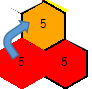
\includegraphics[width=0.15\textwidth]{content/pictures/attack1.png}
	\label{pic:bild}
	\caption{Spieler-Rot greift Spieler-Orange an}
\end{figure}
 Wir haben nun eine 4, eine 1, eine 3, eine 6, und eine 3 gew�rfelt. Somit
 ergibt sich eine Summe von 17. Diese Summe ist ausschlaggebend. Wenn der Gegner
 mit seinen 5 W�rfeln unsere Summe schlagen kann, haben wir verloren und unser
 Angriff war erfolglos. In diesem Fall kann unser Gegner und wir h�chstens 6 + 6
 + 6 + 6 + 6 W�rfeln. Also eine 30. Unser Gegner w�rfelt jedoch nur eine 10.
 Somit haben wir eine h�here Zahl und dieses Feld geh�rt uns.
 \begin{figure}[!htbp]
	\centering
	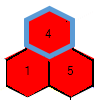
\includegraphics[width=0.15\textwidth]{content/pictures/attack2.png}
	\label{pic:bild}
	\caption{Spieler-Rot �bernimmt Spieler-Orange Feld}
\end{figure}
 Wenn wir das Feld eingenommen haben, bleibt ein W�rfel auf den Feld, von dem
 wir, angegriffen haben. Somit bleibt dieses Feld in unserem Besitz. Da wir das
 feindliche Feld �bernommen haben, wandern die anderen 4 W�rfel auf das besiegte
 Feld. Nat�rlich wechselt dieses Feld auch die Farbe.\\\\
 Wenn ein Angriff erfolglos war und wir eine kleinere Summe haben als der
 Gegner, dann verlieren wir alle W�rfel bis auf einen. Dieser eine W�rfel bleibt
 dann auf unserem Feld zur�ck.\\
\begin{figure}[!htbp]
	\centering
	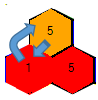
\includegraphics[width=0.15\textwidth]{content/pictures/attack3.png}
	\label{pic:bild}
	\caption{Fehlgeschlagener Angriff}
\end{figure}
 In so einem Fall hat der Gegner leichtes Spiel und kann sobald dieser an der
 Reihe ist einen Konter starten und dieses "geschw�chte" Feld angreifen.\\ \\
 Ein Feld auf dem nur ein W�rfel liegt, kann nicht angreifen. Hier macht es
 keinen Sinn, da wir das eigene Feld verlassen m�ssen. Sprich nur von Feldern
 mit der W�rfelanzahl > 1 kann angegriffen werden.\\ \\
 Ein Spieler muss aber nicht zwangswei�e angreifen. Er kann auch theoretisch
 vorsichtig Spielen und eine Verteidigungslinie aufbauen. Da man wie schon
 erw�hnt nur direkt anliegende Felder angreifen kann, kann man auch W�rfel an
 direkt anliegende Felder verschieben. So kommt auch etwas Taktik in das Spiel.
 Auf diese Art lassen sich Verteidigungs- bzw. Angriffslinien aufbauen. Beim
 Verschieben werden wieder alle W�rfel bis auf einen auf das gew�nschte Feld
 verschoben.\\
 Wenn ein Spieler alle Entscheidungen getroffen hat, kann er seine Runde
 abschlie�en und der n�chste Spieler ist an der Reihe.\\ 
 So hat Spieler f�r Spieler die Chance seine Einheiten zu verschieben bzw.
 gegnerische Felder anzugreifen.\\
 Nachdem alle Spieler am Zug waren ist eine Runde beendet. Nach einer Runde
 bekommt jeder Spieler neue W�rfel auf seine Felder verteilt. So bekommt jeder
 Spieler "Nachschub" f�r seine Felder und kann seine Einheiten wieder neu
 verteilen bzw. andere Felder angreifen.\\ \\
 Ziel ist es die gesamte Spielfl�che mit seinen Einheiten einzunehmen.\\ 
 Am leichtesten lernt man die Spielabl�ufe jedoch beim Spielen. 
 
 

\chapter{Verwendete Technologien}  

Random.org API\\ \\

Um beim W�rfeln richtige und keine Pseudo-Zufallszahlen zu bekommen, 
greifen wir auf die Random.org API zu. Diese liefert Zufallszahlen 
in Abh�ngigkeit vom Weltraumrauschen und wird deshalb von Lotterien, 
Casinos und Online-Spielen benutzt, da es sich um wahre Zufallszahlen handelt 
und nicht um Pseudo-Zufallszahlen, die ein Computer generiert.\\
Die Implementierung findet sich in der Klasse RandomGenerator. 
Diese Klasse enth�lt die �ffentliche Methode "public int rollTheDices(int dices)". 
Diese Methode ruft random.org auf mit passenden �bergabeparametern (kleinst m�gliche Zahl, 
gr��t m�gliche Zahl, Anzahl Zahlen) auf. 
Das Ergebnis (bzw. der HTML Code der Ergebnis-Seite) wird mit der Methode "DownloadData" heruntergeladen. 
Dieser muss dann erst noch geparst werden, also die generierten Zahlen aus dem HTML-Code herausgefilert 
und in einem Integer-Array gespeichert werden. Da es bei diesem Spiel nur um die Summe aller Augenw�rfel geht, 
werden alle Zahlen des Integer-Arrays anschlie�end addiert und die Summe als R�ckgabewert zur�ckgegeben.\\
Sollte dabei ein Fehler auftreten (z.B. weil der Rechner gerade keine Internetverbindung hat),
wird die rekursive Methode "rollTheDiceOffline" aufgerufen, die Pseudo-Zufallszahlen generiert 
und die Summe davon zur�ckgibt. Somit ist man nicht auf eine Internetverbindung beim Spielen angewiesen. 
\chapter{Verwendete Design-Pattern}  

RandomGenerator (Singleton)\\ 

Den Zufallsgenerator, der wahre Zufallszahlen mit Hilfe von der Random.org API generiert, 
haben wir als Singleton implementiert. Von dem RandomGenerator soll es nur eine Instanz geben. 
Man ruft von au�en nur die Methode "rollTheDice" auf (diese generiert dann, 
je nachdem ob man eine Internetverbindung hat oder nicht, 
richtige oder Pseudo-Zufallszahlen und gibt deren Summe zur�ck). 
Mehrere Instanzen eines RandomGenerators anzulegen w�re daher nicht sinnvoll, 
da die Methode "rollTheDice" nie mehrmals parallel aufgerufen werden muss.\\ \\

Builder-Pattern\\ 

Das Builder-Pattern wird bei uns verwendet um das Spielfeld zu erzeugen. Wir
verwenden zweimal das Pattern. Einmal wie erw�hnt f�r das "Board" und einmal
f�r das "BoardState". Das Builder-Pattern ist daf�r da, um die Erstellung
komplexer Objekte zu vereinfachen.\\ \\

DTO-Pattern\\ 

Das DTO-Pattern verwenden wir um Daten zu sammeln und diese dann in die
Datenbank zu speichern. So sammeln wir an verschiedenen Stellen im Code Daten
und in der letzten Form speichern wir diese in die Datenbank.\\
Das DTO-Pattern ist daf�r da, primitive Datentypen abzuspeichern bzw.
einzusammeln.

\newpage
Observer-Pattern\\

Da wir auf dem Spielfeld die W�rfelanzal anzeigen und diese sich st�ndig �ndert,
haben wir hier das Observer-Pattern implementiert. Nachdem jeder Spieler seine
Z�ge gemacht hat, werden W�rfel neu vergeben bzw. auf die Vorhandenen addiert.
Jetzt muss die GUI und alle dazugeh�rigen Objekte aktualisiert werden.\\ 
Durch die Observer-Funktionalit�t lassen sich solche Probleme leicht l�sen.\\ \\

Somit haben wir vier Design-Pattern implementiert. (Gefordert waren hier drei
Pattern)



% Schalgwortverzeichnis (Index)
%\printindex

% Literaturverzeichnis
%\singlespacing
%\bibliographystyle{alphadin} 
%\bibliography{bibtex}

% Eidesstattliche Erklärung


\appendix
% Hier können Anhaenge angefuegt werden

\end{document}      